\documentclass[12pt]{article}
\usepackage[a4paper]{geometry}
\usepackage{graphicx}
\usepackage{cleveref}
\title{Kaggles stroke dataset}
\author{Ciaran Welsh}

\begin{document}

    \maketitle

    \section{Introduction}
    I have trained a feed forward neural network to classify people into stroke victims or not-stroke victims
    based on their age, their average glucose level, hypertension, heart disease, gender, bmi, marital status and
    work type.
    \subsection{Exploration}
    I produced a selection of histograms and PCA plots before deciding that the best way to visualise this data is by
    using scatter matrix plots with kernel density estimators along the diagonal. An example is shown in
    figure \cref{fig:scatter_matrix} which the rest can be found in ./data/Plots/scatter_matrix.

    \section{Preprocessing}
    The biggest problem with this dataset is that the number of stroke samples was much smaller than the number
    of non-stroke samples (98\% vs 2\%). To deal with this problem, I chose to under sample the non-stroke
    data, ensuring the number of stroke and non-stroke samples were equal in both the train and validation data. This turned
    out to be a naive method because it doesn't factor in the impact that age has on stroke incidence. When training
    with this naive method, the model validation score was very unstable between runs and dependent on the
    age distribution of stroke victims. Stratifying the under-sampling such that the age distribution
    within the stroke and non-stroke in both the train and validation data were the same seemed to greatly help with
    this problem. This idea was based on the distribution of stroke incidence with age (\cref{fig:scatter_matrix}).

    \begin{figure}[t]
        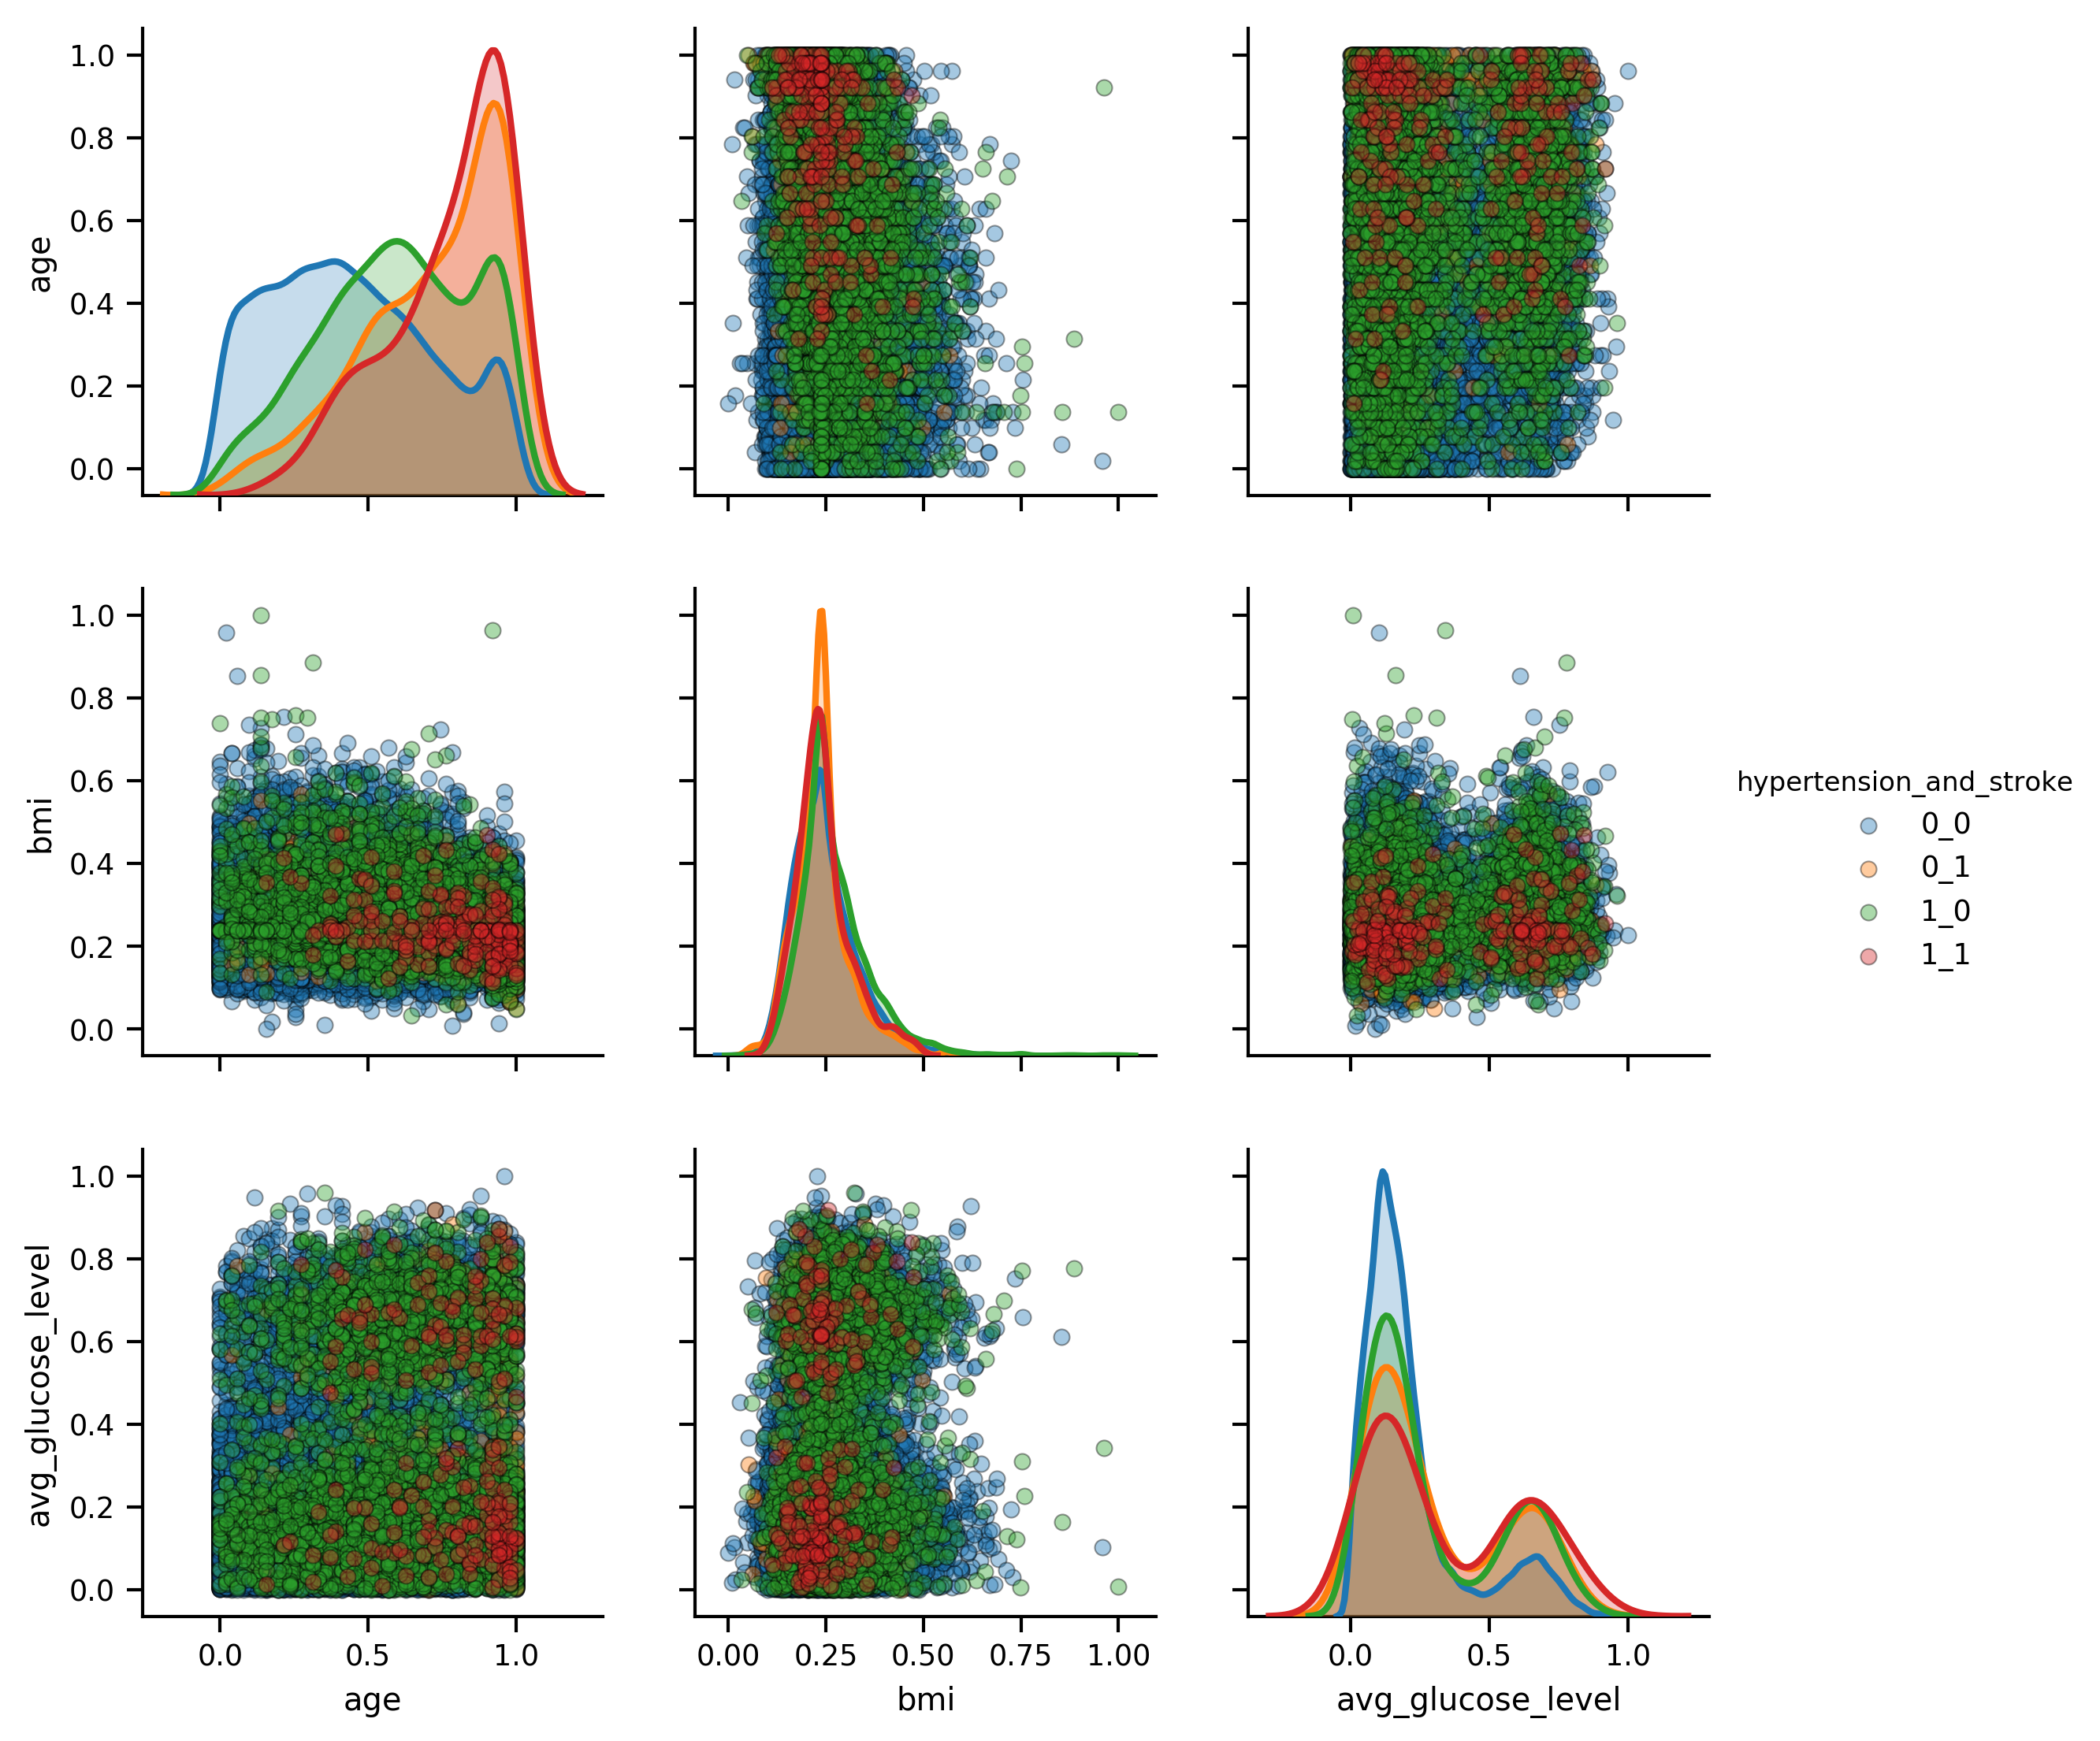
\includegraphics[width=\textwidth]{../data/Plots/scatter_matrix/proc_hypertension.png}
        \caption{Scatter matrix showing relationships between bmi, average glucose levels. This plot is coloured by
        hypertension and stroke}
        \label{fig:scatter_matrix}
    \end{figure}

    Other data preprocessing steps:
    \begin{enumerate}
        \item Discard young data. There are very few people under 30 in this dataset that have had a stroke. Therefore these were removed from the analysis.
        \item Drop the other gender. There are very few `Other' values and none who have had strokes.
        \item Impute the bmi column using the median, since only around 3\% of data were missing this is a reasonable thing to do instead of deleting the sample.
        \item Scale continuous data between 0 and 1 so they exist on a similar scale for fitting
        \item One hot encode categorical variables
        \item convert boolean variables to 1's and 0's
        \item Remove the residence category: exploratory data analysis seems to suggest its not predictor of stroke incidence.
        \item Remove smoking status category. It has too many missing values.
        \item remove any remaining samples with nan values.
    \end{enumerate}

    Note that model performance may still be improved by modifying the preprocessing strategy. Of note there is a
    package called Imbalanced-learn that would be of interest.

    \subsection{Model architecture}
    A simple feedforward network was implemented using the tensorflow interface to keras. Dropout layers were used
    after each dense layer for regularisation and the relu activation funciton was used. The output layer has a single
    neural with a sigmoid activation function and the model was trained by minimizing the binary crossentropy objective
    function using the ADAM optimizer. An early stopping callback was used to prevent overfitting by stopping training
    when the validation accuracy begins to decline. A plot of training history can be found in \cref{fig:training_history}.

    \begin{figure}
        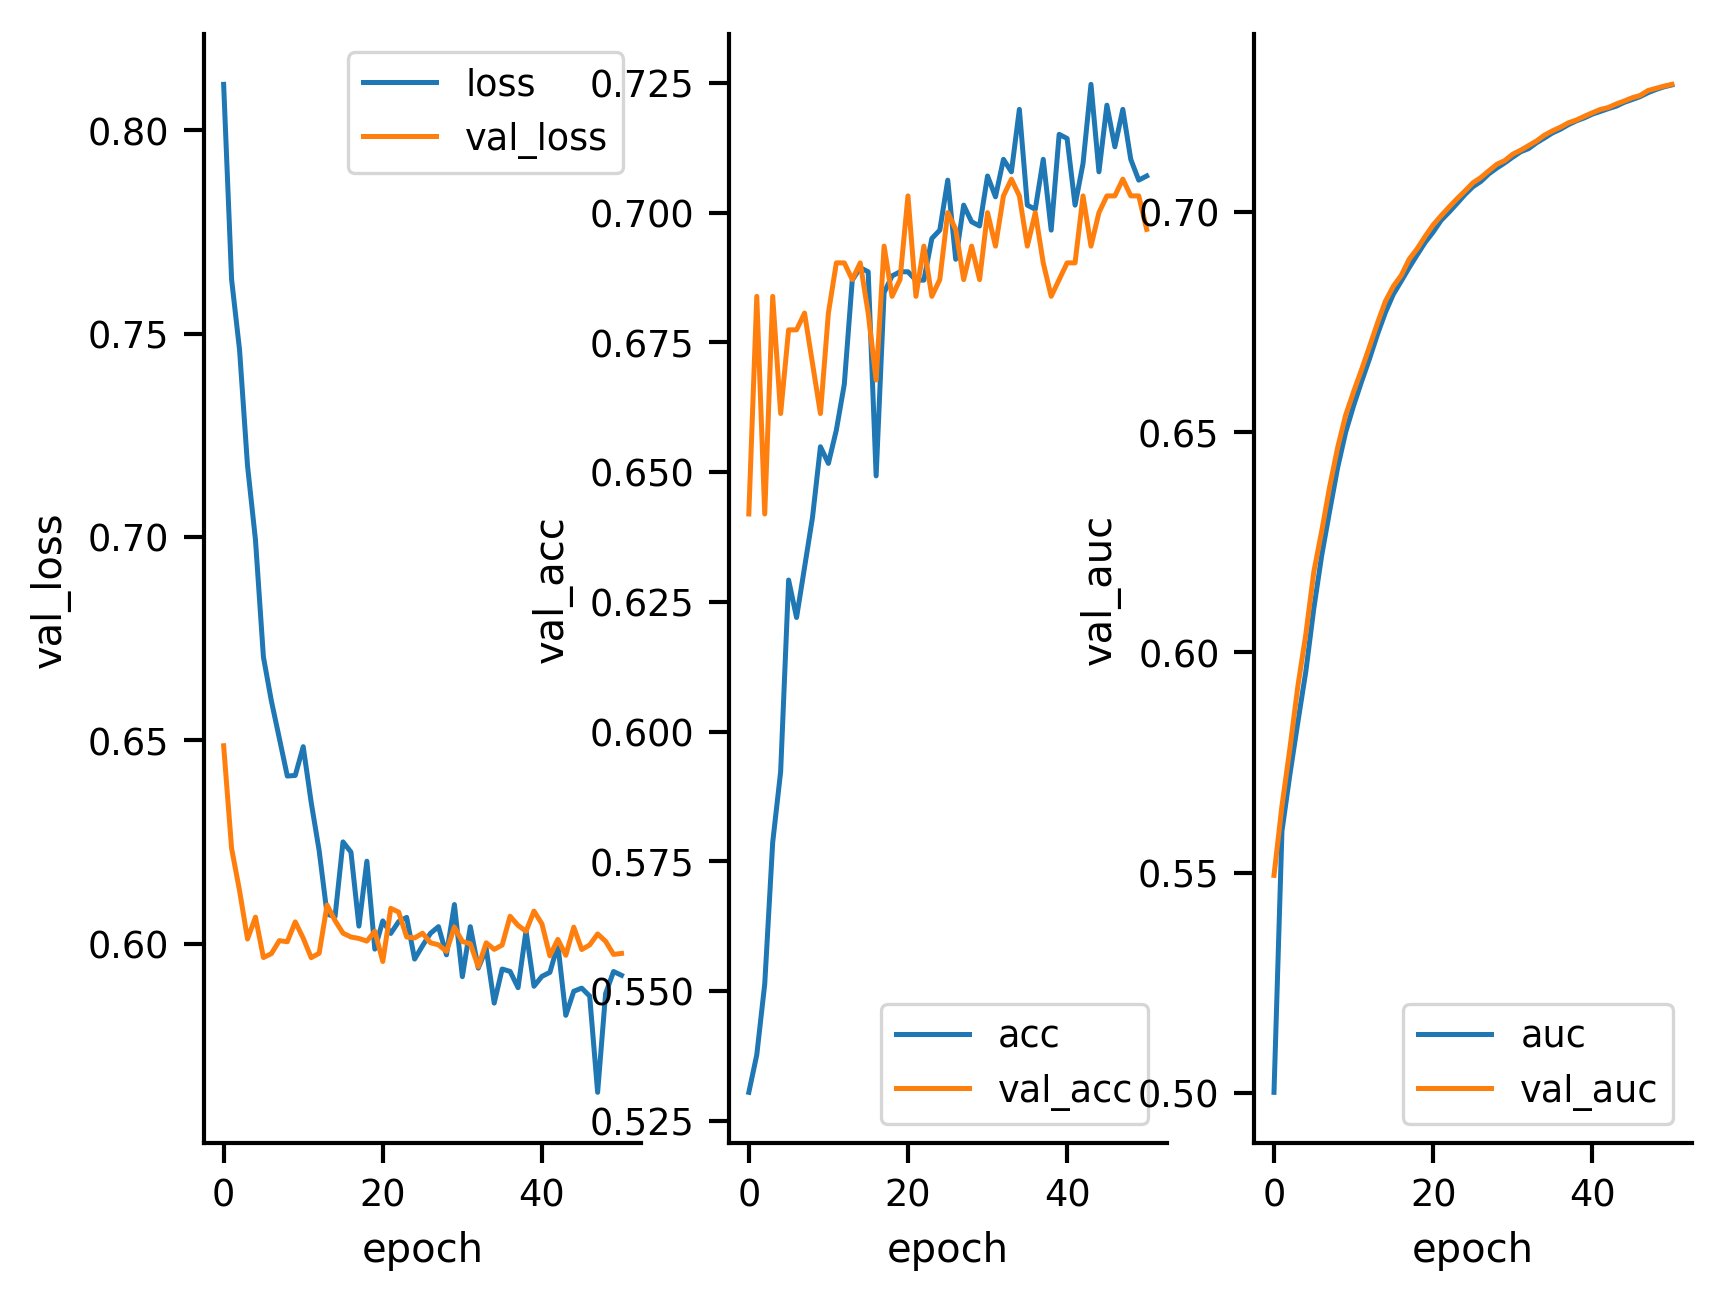
\includegraphics[width=0.75\textwidth]{../data/Plots/history.png}
        \caption{Training history}
        \label{fig:training_history}
    \end{figure}

    \subsection{Model performance}
    Since an under sampling strategy was used to deal with the imbalanced data problem, the model only trains
    with a fraction of the data. To assess the models predictive robustness, a bootstrapping strategy was used (\cref{table:boot}).
    Model train and validation scores were monitored while repeating the model fitting process with a different sample
    from the not-stroke population with the same stroke population. Its possible this decision may have a negative impact
    on model generality due to over fitting the stroke population. As before, sampling was stratified by age group in
    addition to ensuring equal proportions of stroke and not-stroke victim.

    \begin{table}[]
        \begin{tabular}{|l|l|l|l|l|}
            \hline
            & loss & acc & val\_loss & val\_acc \\ \hline
            Average & 0.61 & 0.70 & 0.59 & 0.71     \\ \hline
            Std & 0.013 & 0.014 & 0.020 & 0.029    \\ \hline
        \end{tabular}
        \caption{Average and standard deviations for 100 bootstrap models}
        \label{table:boot}
    \end{table}

    Usually the separate test dataset would be useful in assessing

    \subsection{Things I have run out of time for}
    Time constrains
    - could not tune hyperparameters well
    - many factors can influence this model including groups used for stratification. inclusion of not needed features.
    - all the hyper parameters, model architecture, drop out rates, loss and algorithm choice.

    \subsection{Room for improvement}


\end{document}

% However, I am not convinced that all of these variables are informative for classifying stroke victims.
%    I have already excluded residence as a factor involved in stroke incidence based on the scatter plot (data/Plots/scatter_matrix/raw_Residence_type)
%    but I suspect marital status should be excluded as well. Given more time I would systematically drop each variable
%    in turn and measure its impact on model performance.
%